\documentclass{gd-llncs}
%\documentclass[preprint,3p,12pt]{elsarticle}

\usepackage{graphicx}
\usepackage[]{subfig}
\usepackage{svg}
\usepackage[]{pdfpages}
\graphicspath{{./images/}}
% \journal{Computational Geometry: Theory and Applications}

%\newtheorem{theorem}{Theorem}
%\newtheorem{problem}{Problem}
%\newtheorem{lemma}{Lemma}
%\newtheorem{proposition}{Proposition}
%\newenvironment{proof}{\noindent \emph{Proof}: }{\qed}

\newcommand{\comm}[1]{}
\newcommand{\TODO}[1]{{\color{magenta}{#1}}}
\newcommand{\new}[1]{\textcolor{green}{#1}}
%\newcommand{\note}[1]{\textcolor{blue}{[#1]}}

\newcommand{\df}[1]{\mbox{\textbf{#1}}}
\def\Cost{\text{\emph{routing cost}}}
\def\aCost{\text{\emph{additional cost}}}
\newcommand{\gv}{\widetilde{G}}
\newcommand{\ink}{I}
\newcommand{\cc}{C}
\newcommand{\inkcoeff}{k_{\textit{ink}}}
\newcommand{\lencoeff}{k_{\textit{len}}}
\newcommand{\capcoeff}{k_{\textit{cap}}}
\DeclareMathOperator{\nul}{\textit{null}}
\begin{document}


\title{Browsing large graphs with MSAGLJS, a graph draph drawing tool in JavaScript }
\author{%
  Lev Nachmanson  \and
  Xiaoji Chen
}%
\institute{
  Microsoft Research, US,\\
  \email{levnach@hotmail.com, cxiaoji@gmail.com},\\
  Msagljs github home page:
  \texttt{https://github.com/microsoft/msagljs}
}
\maketitle
%\ead{levnach@microsoft.com}
%\address[LN]{Microsoft Research, USA}

%\ead{spupyrev@gmail.com}
%\address[SP]{Ural Federal University, Russia}

\begin{abstract}
  There has been progress in visualization of large graphs recently. Still, interacting with a large graph in the browser with the same ease as browsing an online map, inspecting the high level structure and zooming to the lower details, is still an unsolved problem, in our opinion. In this paper we describe MSAGLJS's approach to two aspects of this problem. Firstly, we give a novel algorithm for edge routing, where the edges do not overlap the nodes. The algorithm does not necesserely creates optimal paths but is efficient and creates visually appealing paths. Secondly, to facilitate graph vizualization with DeckGL, namely fast zoom-\(in/out\), and pan operations, and keeping the number of entities on the screen below a specific bound, we use tiling. Our tiling procedure is simple and efficient. It is the second contribution of the paper.
\end{abstract}






\section*{Introduction}

\label{sec:intro}
\section*{Related work}
Links to large graph visualization


\cite{graphexp}

\cite{graphviz}

\cite{regraph}

\cite{skewed}

\cite{circos}

\cite{gibson2013survey}

machine learing approach
\cite{kwon2017would}

\cite{lin2013interactive}

\cite{cosmograph}

\section*{Edge routing}
The edge routing starts as in~\cite{dwyer2010fast}, by building a spanner graph, an approximation of the full visibility graph. The spanner, see Fig.~\ref{fig:spanner}, is built on a Yao graph, which was introduced independently by Flinchbaugh and Jones~\cite{flinchbaugh1981strong}  and Yao~\cite{yao1982constructing}. A Yao graph is defined by the set of cones with the apices at the vertices. The cones have the same angle, usually in the form of $\frac{2\pi} {n}$, where $n$ is a natural number. This way the cones with the apex at a specific vertex partition the plane as illistrated in as illistrated in Fig.~\ref{fig:yao}. For each cone at most one edge is selected connecting the cone apex with a vertex inside of the cone.

\begin{figure}[]
  \centering
  \begin{minipage}[b]{0.5\textwidth}
    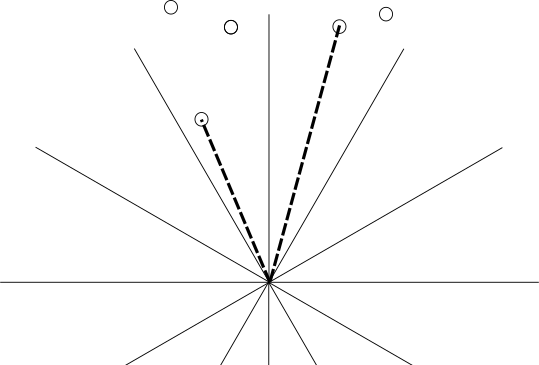
\includegraphics[width=\textwidth]{yao.pdf}
    \caption{\small{Fragment of a Yao graph}}
    \label{fig:yao}
  \end{minipage}

  \vfill
  \begin{minipage}[b]{\textwidth}
    \includesvg[width=\textwidth]{visibility_graph.svg}
    \caption{\small{Spanner graph is built using the idea of Yao graphs. The dashed curves are the original node boundaries. Each original curve is surrounded by a polygon with some offset to allow the polyline paths smoothing without intersecting the original curves. \\
        The edge marked by the circles is created because the top vertex is inside of the cone and is the closest among such vertices to the cone apex. The apex of the cone is the lower vertex of the edge. \\MSAGLJS uses cone angle $\frac{\pi}{6}$. This gives paths with lengths not that are not greater than the optimal length divided by $\cos(\frac{\pi}{12})$}}
    \label{fig:spanner}
  \end{minipage}

\end{figure}


The approach of~\cite{dwyer2010fast}, first builds a polyline on the spanner, and then applies some local modifications to shorten the polyline and to make it smooth. For shortening it tries to shortcut a vertex, as illustrated in Fig~\ref{fig:shortcut}. To make it smooth it inscribed Bezier segment into the polyline corners. While anylyzing performance of edge routing in MSAGLJS, we noticed that for a graph with more than 10000 edges these heuristics become the major bottleneck.
\begin{figure}[!tbp]
  \centering
  \begin{minipage}[b]{0.4\textwidth}
    \includegraphics[width=\textwidth]{./naive_shorcut_now_working.png}

    \caption{Unsuccessful shortcut}
  \end{minipage}
  \hfill
  \begin{minipage}[b]{0.4\textwidth}
    \includegraphics[width=\textwidth]{fillet_corner.png}
    \caption{Fitting a Bezier segment into a polyline corner}
  \end{minipage}
  \caption*{Inefficient local improvements}
\end{figure}

\label{fig:shortcut}

The reason for this was that we queured if a lines intersects any entity of the graph. Even by optimizing this operations by using R-Trees~\cite{guttman1984r}, we saw that about \%90 of the edge routing running time was spent on these heuristics. Another disadvantage of the naive shortcutting of polyline corners is that often in the case of the failure, when a shortcut is not found, the resulting path is not visually appealing.


\comm{
  \section{Further Examples}
}
\bibliography{main}
\bibliographystyle{ieeetr}
\end{document}
